\documentclass[11pt, twocolumn]{article}

\usepackage[spanish]{babel}
\usepackage[none]{hyphenat}
\usepackage[left=1.5cm, right=1.5cm, top = 2cm, bottom=2.5cm]{geometry}
\usepackage{parskip}
\usepackage[export]{adjustbox}
\usepackage{enumitem}
\usepackage{listings}
\usepackage{color}
\usepackage{fancyhdr}
\usepackage{graphicx}
\usepackage{caption}
% \usepackage{subcaption}
% \usepackage{wrapfig}
% \usepackage{longtable}
% \usepackage{multirow, makecell}
% \usepackage{amsmath} 
\usepackage[hidelinks]{hyperref}
\usepackage{csquotes}

\newcommand{\linejump}{\hfill \break}
\renewcommand{\thefootnote}{\fnsymbol{footnote}}
% \newcommand{\unit}[1]{\ensuremath{\, \mathrm{#1}}}

\definecolor{dkgreen}{rgb}{0,0.6,0}
\definecolor{gray}{rgb}{0.5,0.5,0.5}
\definecolor{mauve}{rgb}{0.58,0,0.82}
\lstset{
  language=Java,
  aboveskip=3mm,
  belowskip=3mm,
  showstringspaces=false,
  columns=flexible,
  basicstyle={\tiny\ttfamily},
  numbers=none,
  numberstyle=\tiny\color{gray},
  keywordstyle=\color{blue},
  commentstyle=\color{dkgreen},
  stringstyle=\color{mauve},
  breaklines=true,
  breakatwhitespace=true,
  tabsize=2
}

\sloppy
\setlength{\parindent}{0cm}
\setlength{\columnsep}{0.5cm}
\decimalpoint
\graphicspath{{img/}}

\hypersetup{colorlinks=true, urlcolor=blue, citecolor=blue}
\urlstyle{same}

\pagestyle{fancyplain}
\fancyhf{}
\fancyhead[L]{\scriptsize 
  Universidad Nacional Autónoma de México \\
  Laboratorio de Programación Orientada a Objetos \\
  M.C. Leonardo Ledesma Dominguez
}
\fancyhead[R]{\thepage}


\begin{document}
  \twocolumn[
    \centering
    Acosta Porcayo Alan Omar, Gutiérrez Grimaldo Alejandro, Medina Villa Samuel

    \linejump

    \LARGE \textbf{Práctica 5. Abstracción y Encapsulamiento} \\
    
    \linejump
  ]
      
  \footnotetext{
    \scriptsize 
    Acosta Porcayo Alan Omar Ing. en Computación 320206102 \\
    Gutiérrez Grimaldo Alejandro Ing. en Computación 320282098 \\
    Medina Villa Samuel Ing. en Computación 320249538
  }
        
  \fancyfoot{}

  \section*{Resumen}


  \section*{Introducción}
  

  \section*{Objetivos}
  \begin{itemize}
    \item 
  \end{itemize}

  \section*{Metodología} 
  \subsection*{Ejercicio realizado por el profesor}
  Ejemplo de uso de interfaces. 

  \textbf{Código}
  \begin{lstlisting}
interface Poligono {
  // firma de metodos
  void getArea(int a, int b);
}  

class Rectangulo implements Poligono {
  // implementacion del metodo de la interfaz
  public void getArea(int a, int b) {
    System.out.println("El area del rectangulo es: " + (a * b));
  }
}

class Main {
  public static void main(String[] args) {
    Rectangulo r = new Rectangulo();
    r.getArea(4, 8);
  }
}  
  \end{lstlisting}

  Recreación del juego ``Gato''.
  \begin{lstlisting}
import java.util.*;

interface Board {
  // En interfaz por lo general los metodos son default
  String checkWinner();
  void printBoard();
}

public class TicTacToe implements Board {
  static String[] board;
  static String player; // Posible objeto que venga de la clase Player L11
    
  // Override
  public String checkWinner() {
    for(int i = 0;  i <8; i ++) {
      String line = null;
      switch(i) {
        case 0: line = board[0] + board[1] + board[2]; break;
        case 1: line = board[3] + board[4] + board[5]; break;
        case 2: line = board[6] + board[7] + board[8]; break;
        case 3: line = board[0] + board[3] + board[6]; break;
        case 4: line = board[1] + board[4] + board[7]; break;
        case 5: line = board[2] + board[5] + board[8]; break;
        case 6: line = board[0] + board[4] + board[8]; break;
        case 7: line = board[2] + board[4] + board[6]; break;
      }

      if(line.equals("XXX")) // Si gana el jugador X
				return "X";
			else if(line.equals("OOO")) // Si gana el jugador O
				return "O";
    }

    for(int a = 0; a < 9; a ++) {
      if(Arrays.asList(board).contains(String.valueOf(a + 1)))
          break;
      else if(a==8)
          return "DRAW";
    }

    System.out.println("\nEs el turneo de " + player + ", ingrese una casilla: ");

    return null;
  }

  //imprimir
  /*
  |-------|-------|-------|
  |	  1	  |	  2  	|  	3  	|
  |-------|-------|-------|
  |	  4	  |	  5	  |	  6	  |
  |-------|-------|-------|
  |	  7	  |	  8  	|  	9  	|
  */

  public void printBoard() {
    System.out.println("\n|---|---|---|");
    System.out.println("| " + board[0] + " | " + board[1] + " | " + board[2] + " |");
    System.out.println("|---|---|---|");
    System.out.println("| " + board[3] + " | " + board[4] + " | " + board[5] + " |");
    System.out.println("|---|---|---|");
    System.out.println("| " + board[6] + " | " + board[7] + " | " + board[8] + " |");
    System.out.println("|---|---|---|");
  }

  public static void main(String[] args) {
    Scanner in = new Scanner(System.in);
    board = new String[9];
    player = "X";
    String winner = null;

    TicTacToe t = new TicTacToe();

    // Llenar la matriz board
    for(int i=0;i<9;i++)
      board[i] = String.valueOf(i+1);

    System.out.println("Bienvenido Tic Tac Toe 3x3");

    t.printBoard();

    System.out.println("Es el turneo de " + player + ", ingrese una casilla: ");
    while(winner == null) {
      int numSlot;

      numSlot = in.nextInt();
      if(!(numSlot>0 && numSlot<=9)) {
        System.out.println("Opcion no valida");
        continue;
      }

      if(board[numSlot-1].equals(String.valueOf(numSlot))) {
        board[numSlot-1] = player; // Player vale "X"
        if(player.equals("X"))
          player = "O";
        else
          player = "X";
        t.printBoard();
        winner = t.checkWinner();
      } else
        System.out.println("El slot ya esta ocupado");
    }

    if(winner.equals("DRAW"))
      System.out.println("Nadie gana. Gracias por jugar");
    else 
      System.out.println("Ganaste " + winner + " eres un PRO");

    in.close();
  }
}
  \end{lstlisting}

  \section*{Resultados}
  \subsection*{Problema 1}
  Modifique el programa de \textit{Tic Tac Toe} haciendo: 
  \begin{enumerate}[label=\alph*.]
    \item El Juego de $5\times 5$ y el que gane lo haga con $4$ símbolos unidos.
    \item Cree una clase abstracta que sea el jugador (X-O) y herede la clase principal.
  \end{enumerate}
  \textbf{\textit{Implementar la herencia hibrida, usar interfaces y clases abstractas.}}

  \linejump
  \textbf{Explicación} \\


  \textbf{Código}
  % \begin{lstlisting}
    
  % \end{lstlisting}

  \textbf{Ejecución}
  % \begin{figure}[ht]
  %   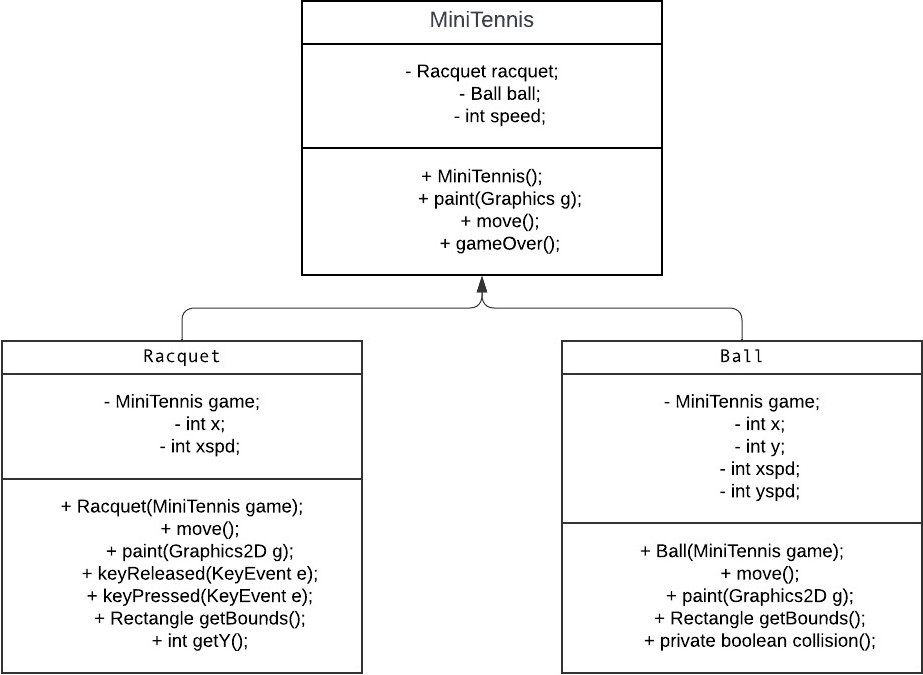
\includegraphics[width=\columnwidth, center]{P1.jpg}
  % \end{figure}

  \subsection*{Problema 2}
  Realice un verificador de contraseña usando encapsulamiento de tipo \textit{private} y \textit{protected}. El programa recibe una cadena candidata para ser contraseña y se valida que:
  \begin{enumerate}[label=\alph*.]
    \item Tenga entre 8 y 16 de caracteres
    \item Que tenga al menos un carácter especial.
    \item Que tenga al menos un número.
    \item Que tenga al menos una letra minúscula.
    \item Que tenga al menos una letra mayúscula.
  \end{enumerate}
  Investigue como se hace para ocultar los caracteres escritos en la consola.

  Al final regrese si la contraseña es débil, mediana o fuerte.

  \textbf{\textit{Implementar encapsulamiento privado y protegido.}}

  \linejump
  \textbf{Explicación} \\


  \textbf{Código}
  % \begin{lstlisting}
    
  % \end{lstlisting}

  \textbf{Ejecución}
  % \begin{figure}[ht]
  %   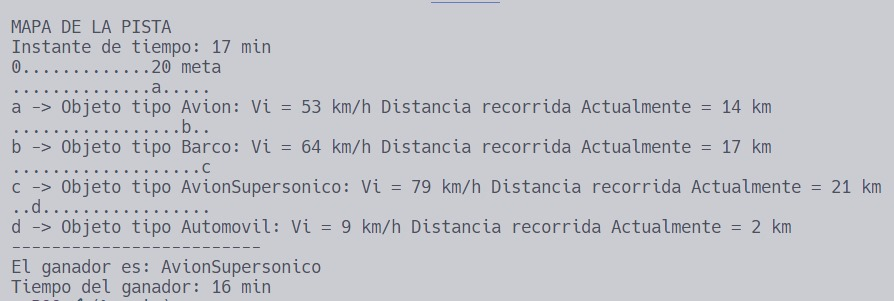
\includegraphics[width=\columnwidth, center]{P2.jpg}
  % \end{figure}

  \subsection*{Problema 3}
  Programa un ahorcado utilizando la composición de objetos:
  \begin{enumerate}[label=\alph*.]
    \item La palabra adivinanza tiene que ser seleccionada de manera aleatoria de un arreglo de mínimo 30 palabras.
    \item El ahorcado deberá mostrarte en consola con una figura simple por ejemplo
    
    Palabra oculta: “MATEMATICAS” \\
    Adivina: $\_$ $\_$ $\_$ $\_$ $\_$ $\_$ $\_$ $\_$ $\_$ $\_$ $\_$

    \begin{figure}[ht]
      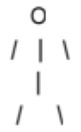
\includegraphics[width=0.15\columnwidth, center]{ahorcado.png}
    \end{figure}
    \item Si el usuario gana mostrar un mensaje de ganador y de la misma manera si se pierde.
    \item Considere las clases:
    \begin{enumerate}[label=\roman*.]
      \item Palabra (palabras ocultas)
      \item Ahorcado (figura)
      \item \textit{Main} (se programa la lógica del juego)
    \end{enumerate}
  \end{enumerate}

  \textbf{\textit{Implementar composición de objetos.}}

  \linejump
  \textbf{Explicación} \\


  \textbf{Código}
  % \begin{lstlisting}
    
  % \end{lstlisting}

  \textbf{Ejecución}
  % \begin{figure}[ht]
  %   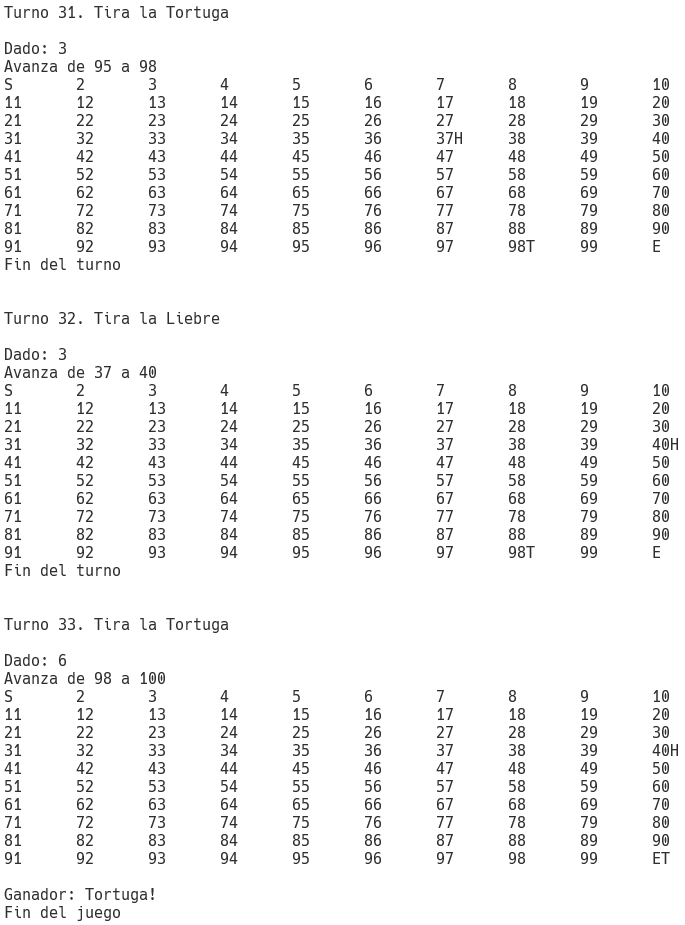
\includegraphics[width=\columnwidth, center]{P3.jpg}
  % \end{figure}

  \subsection*{Problema 4}
  El matemático S. Ulam en 1964 planteo una secuencia de números entera que sigue una serie de reglas planteada en \url{https://edabit.com/challenge/RkicZ4kkcSx8K3d4e}x. Programe la secuencia de Ulam, pero que reciba desde consola los primeros dos elementos de la secuencia y se calcule sobre esos dos elementos.

  Por ejemplo:
  \begin{figure}[ht]
      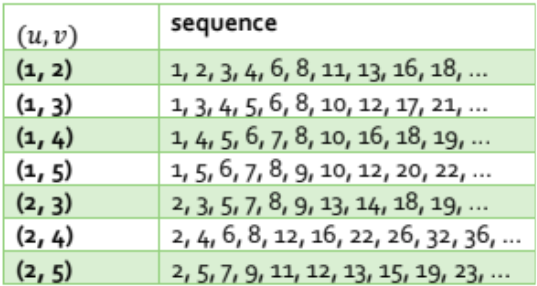
\includegraphics[width=0.8\columnwidth, center]{secuencia.png}
  \end{figure}

  \textbf{\textit{Para manejar la secuencia haga uso de ArrayList exclusivamente.}}

  \linejump
  \textbf{Explicación} \\


  \textbf{Código}
  % \begin{lstlisting}
    
  % \end{lstlisting}

  \textbf{Ejecución}
  % \begin{figure}[ht]
  %   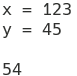
\includegraphics[width=\columnwidth, center]{P4.jpg}
  % \end{figure}

  \section*{Conclusiones}
  

  \section*{Referencias}
  \small
  Solano, J. (2017, 20 enero). \textit{Manual de prácticas de Programación Orientada a Objetos}. Laboratorio de Computación Salas A y B. \url{http://lcp02.fi-b.unam.mx/} \\

  Matt. \textit{Ulam Sequence}. Edabit. \url{https://edabit.com/challenge/RkicZ4kkcSx8K3d4e}
\end{document}